\section[BibTeX]{BibTeX}



\subsection[Welcome to BibTeX]{Welcome to BibTeX}

\begin{frame}  \frametitle{Why use BibTeX?}
There are a number of very good reasons to use BibTeX instead of manual creation of bibliographies.
\begin{itemize}
\item Automatic creation of bibliographies.
\item Easily change bibliographic styles.
\item Identification of missing sources referenced in text.
\end{itemize}
\end{frame}

\begin{frame}  \frametitle{How BibTeX works}
There are three steps that LaTeX and BibTeX take to make a bibliography.
\begin{itemize}
\item When you typeset a document with citations (e.g. {\color{command}$\backslash$cite{\color{braces}$\{$}{\color{black}zotova}{\color{braces}$\}$}}), LaTeX makes note of each citation.
\item BibTeX takes this list and looks for each reference in a database of publications.
\item Then we tell LaTeX to make the bibliography of all of those publications it found that we referenced.
\end{itemize}
The most time consuming part is initially building the database. After that, you can reference this same database over and over again and BibTeX becomes a breeze.
\end{frame}

\begin{frame}  \frametitle{BibTeX material}
\begin{itemize}
\item Creating your database
\item Citing a reference
\item Typesetting with BibTeX
\item Building style files
\end{itemize}
\end{frame}

\subsection[Building the database]{Building the database}

\begin{frame}  \frametitle{Sample reference entry}
We want to create a reference, similar to the following, for each of the item we want to cite.

\vspace{7mm}

@article$\{\overbrace{\text{zotova}}^{label}$, \\
\hspace{3mm}	Author = $\{$Elena Zotova and Charles D Woody and Ehud Gruen$\}$, \\
\hspace{3mm}	Journal = $\{$Brain Research$\}$, \\
\hspace{3mm}	Pages = $\{$66-78$\}$, \\
\hspace{3mm}	Title = $\{$Multiple representations ... [etc etc].$\}$, \\
\hspace{3mm}	Volume = $\{$868$\}$, \\
\hspace{3mm}	Year = $\{$2000$\}\}$ \\
\end{frame}

\begin{frame}  \frametitle{Make up of a reference}
Each reference needs a publication type (e.g. article, book), and each reference includes many fields. For instance, the following are \textbf{required} and \textit{optional} fields of an article entry.
\begin{center}
\begin{tabular}{lllrr}
\multicolumn{5}{l}{\textbf{label}: The reference label.} \\
\textbf{Author} & \textbf{Journal} & \textbf{Title} & \hspace{5mm} & \\
\textbf{Year} & \textit{Volume} & \textit{Number} \\
\textit{Pages} & \textit{Month} & \textit{Note}
\end{tabular}
\end{center}
A formal list of the available publication types and also which items are required and optional for each type, see
\begin{itemize}
\item[]\color{highlight}http://www.image.ufl.edu/help/latex/entry\_bibtex.shtml
\end{itemize}
\end{frame}

\begin{frame}  \frametitle{An alternative}
If you don't want to build your data base up in such a bare-bones manner, you might try
\begin{itemize}
\item BibDesk: Macs.
\item JabRef: Macs, PCs, Linux.
\end{itemize}
Both of these programs are free and available online. Others exist, and I have only personally used BibDesk.
\end{frame}

\begin{frame}  \frametitle{If you do manage your own...}
Some things you should know if you do not use a program manager:
\begin{itemize}
\item Always include a label, which is how LaTeX identifies the entry.
\item The entry (publication) type and field names are NOT cap-sensitive.
\item Enclose the text for each field (e.g. the author names) in curly braces.
\item You can add extra fields that are not listed and these will be ignored (e.g. if you add an Abstract field to a reference, BibTeX will just ignore it).
\end{itemize}
\end{frame}

\begin{frame}  \frametitle{Special cases}
Giving author names in a non-ambiguous form is sometimes difficult.
\begin{itemize}
\item Always type names as $\{$Given Names Surnames$\}$ or $\{$Surname, Given Names$\}$.
\item Anything enclosed in braces will be treated as a single item (e.g. Author = {\color{braces}$\{${\color{black}Maria} $\{${\color{black}San Martino}$\}\}$}).
\item If there is more than one author, separate each author name by the word \textit{and}. If \textit{and} is part of someone's name, enclose their entire name in braces.
\item You may add accents (e.g. G$\ddot{\text{o}}$del via \texttt{G$\{\backslash$"o$\}$del}).
\end{itemize}
Many other nuances exist. If you encounter a peculiar name, do a little online searching to see how best to put it into the data base.
\end{frame}

\begin{frame}  \frametitle{Abbreviating journal names}
Sometimes you don't want your entry to include the entire journal name. To shorten it, use the \textit{string} entry type:
\begin{itemize}
\item[] @string$\{$JSS = $\{$Journal of Statistical Software$\}\}$
\end{itemize}
These string entries must be defined in the database above where they are used.
\end{frame}

\subsection{Citing a reference}

\begin{frame}  \frametitle{Citing a reference}
There are four commands that can be used.
\begin{itemize}
\item {\color{command}$\backslash$cite\color{braces}$\{${\color{black}labelName}$\}$} [referenceNumber], e.g. [1].
\item {\color{command}$\backslash$citet\color{braces}$\{${\color{black}labelName}$\}$} Surname (year), e.g. Zotova et al. (2000).
\item {\color{command}$\backslash$citep\color{braces}$\{${\color{black}labelName}$\}$} (Surname, year), e.g. (Zotova et al., 2000).
\item {\color{command}$\backslash$nocite\color{braces}$\{${\color{black}labelName}$\}$} Not cited but will show up in bibliography.
\end{itemize}
The first and last work with the \texttt{\color{highlight}uclathes} class. The second two are used in the \texttt{\color{highlight}natbib} package (highly recommended for non-thesis papers).
\end{frame}

\begin{frame}  \frametitle{Other commands in your document}
The following two lines of code must be inserted at the place where the bibliography is to be added:
\begin{itemize}
\item[] {\color{command}$\backslash$bibliographystyle\color{braces}$\{${\color{black}yourStyle}$\}$}
\item[] {\color{command}$\backslash$bibliography\color{braces}$\{${\color{black}databaseName}$\}$}
\end{itemize}
The style command can be moved higher (it doesn't matter). If you use the \texttt{\color{highlight}natbib} package, then you must add it with the other packages:
\begin{itemize}
\item[] {\color{command}$\backslash$usepackage\color{braces}$\{${\color{black}natbib}$\}$}
\end{itemize}
I have not gotten this package to work with the UCLA thesis template.
\end{frame}

\subsection{Typesetting}

\begin{frame}  \frametitle{Making the bibliography}
If you have made your reference database, made citations, and inserted the bibliography commands in your text, then you are ready to create the bibliography. In TeXShop, there are a few simple steps to finish:
\begin{itemize}
\item Typeset your LaTeX document as usual.
\item Change the Typesetting option from LaTeX to BibTeX:

\vspace{1mm}

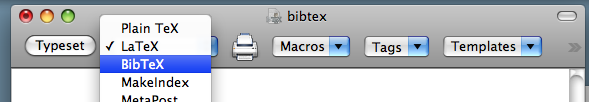
\includegraphics[height=15mm]{bibtex/bibtexTypeset}\hspace{4mm}{}

\item Typeset again with BibTeX.
\item Return the Typesetting option back to LaTeX and compile \textbf{twice} more.
\end{itemize}
\end{frame}

\subsection{Building your own style file (the easy way)}

\begin{frame}  \frametitle{Building a style file}
One of the big benefits of BibTeX is the ability to quickly change the bibliography style and within-text citations. To do this, we use the program {\color{highlight}custom-bib}. Download it at
\begin{itemize}\small 
\item[] \color{highlight} http://www.ctan.org/tex-archive/help/Catalogue/entries/custom-bib.html
\end{itemize}
custom-bib has been included in the {\color{highlight}latexTemp} zip file from the first class.
\end{frame}

\begin{frame}  \frametitle{Building a style file}
Open \texttt{latexTemp} $>$ \texttt{custom-bib}, and open the \texttt{\color{highlight}makebst.tex} file. To run the program,
\begin{itemize}
\item[(1)] Open the file and typeset it.
\item[(2)] Type \texttt{YES} to the first question to get extra directions.
\item[(3)] Choose an appropriate file name (no need to add the extension).
\item[(4)] Answer each of the style questions.
\item[(5)] For the last question, \textit{Finished!! ...  Shall I now run this batch job? (NO)}, type \texttt{YES}.
\end{itemize}
Find and copy the file you named in step (3) with extension \texttt{.bst}. Put it in the folder with whatever files for which you will make a bibliography with this style or in your bibliography folder (however you reference it in your LaTeX document).
\end{frame}

\subsection{Practice}

\begin{frame}  \frametitle{Practice}
Open the \texttt{\color{highlight}latexTemp.tex} file and go to the last section. Add a bibliography reference of {\color{command}$\backslash$citet}{\color{braces}$\{${\color{black}victor}$\}$}. Also add a reference with {\color{command}$\backslash$citep}{\color{braces}$\{${\color{black}victor}$\}$} and typeset (all four steps). What is the difference between your references? How would you use each in a paper?\end{frame}



